

\section{FPGA}
	\subsection{Hardware}
	\begin{frame}{FPGA - Hardware - Visão Geral}
		\begin{itemize}
			\setlength\itemsep{1.5em}
			\item Nos FPGAs, sua configuração é totalmente \textbf{volátil}
			\begin{itemize}
				\setlength\itemsep{1em}
				\item O projeto deve ser \textbf{recarregada} sempre que é \textbf{ligada};
				\item Para isso, a configuração é normalmente guardada numa memória não volátil como a EEPROM.
			\end{itemize}

			\item Internamente:
			\begin{itemize}
				\setlength\itemsep{1em}
				\item Consiste num \textbf{arranjo de blocos lógicos} e \textbf{canais de roteamento}.

				\item Significa que é capaz de alterar seus caminhos de dados/fluxos \textbf{habilitando/desabilitando módulos} \cite{moreira2008}.
			\end{itemize}
		\end{itemize}
	\end{frame}


	\begin{frame}{FPGA - Hardware - Visão Geral}
		\begin{figure}[h]
			\centering
			\caption{``FPGA é um \textit{quadro negro} que pode ser \textit{desenhado} qualquer circuito digital''.}
			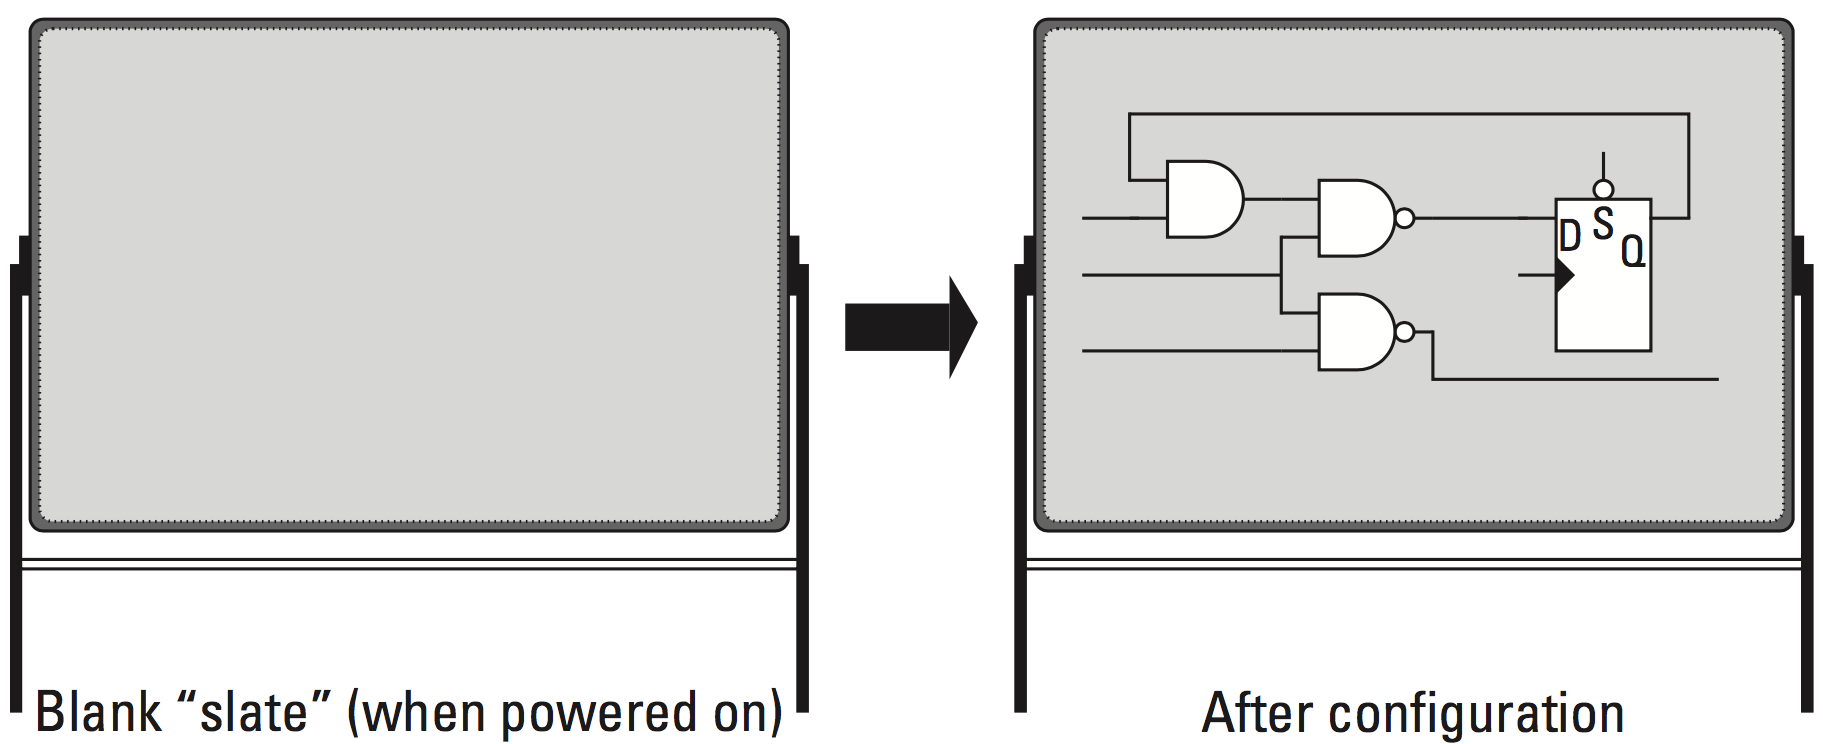
\includegraphics[height=0.7\textheight]{img/fpga/quadro.png}
			\label{fig:quadro}
		\end{figure}
	\end{frame}

	\begin{frame}{FPGA - Hardware - Roteamento de Blocos}
		\begin{multicols}{2}
			\begin{figure}[h]
				\centering
				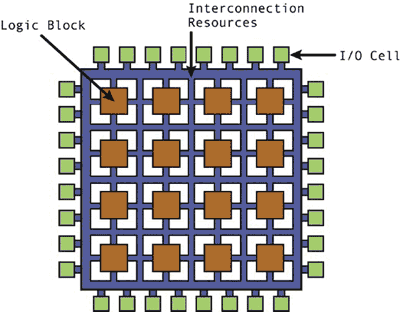
\includegraphics[width=0.5\textwidth]{img/fpga/exempo-simples.png}
				\caption{Exemplo de roteamento interno.}
				\label{fig:exempo-simples}
			\end{figure}
			\columnbreak
			Três módulos:
			\begin{itemize}
				\setlength\itemsep{1.8em}
				\item Blocos de Entrada e Saída;

				\item Blocos Lógicos Configuráveis;

				\item Chaves de Interconexão.
			\end{itemize}
		\end{multicols}
	\end{frame}

	\begin{frame}{FPGA - Hardware - Roteamento de Blocos}
		\begin{multicols}{2}
			\begin{figure}[h]
				\centering
				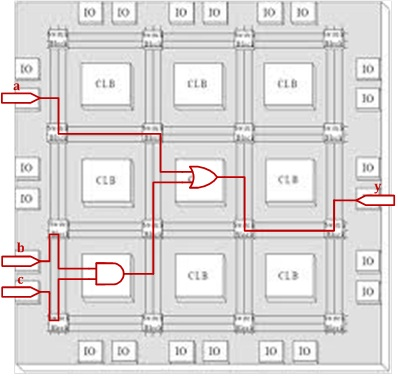
\includegraphics[width=0.45\textwidth]{img/fpga/exemplo.jpg}
				\caption{Outro exemplo de roteamento interno no FPGA.}
				\label{fig:exemplo}
			\end{figure}
			\columnbreak
			Três módulos:
			\begin{itemize}
				\setlength\itemsep{1.8em}
				\item Blocos de Entrada e Saída;

				\item Blocos Lógicos Configuráveis;

				\item Chaves de Interconexão.
			\end{itemize}
		\end{multicols}
	\end{frame}

	\begin{frame}{FPGA - Hardware - Roteamento de Blocos}
		\begin{figure}[H]
			\centering
			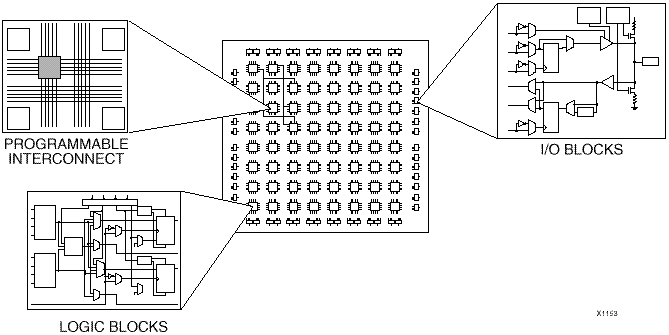
\includegraphics[width=0.97\textwidth]{img/fpga/demonstracao_2.png}
			\caption{Demonstração mais complexa de síntese.}
		\end{figure}
	\end{frame}


	\begin{frame}{FPGA - Hardware - Roteamento de Blocos}
		\begin{multicols}{2}
			\begin{figure}[h]
				\centering
				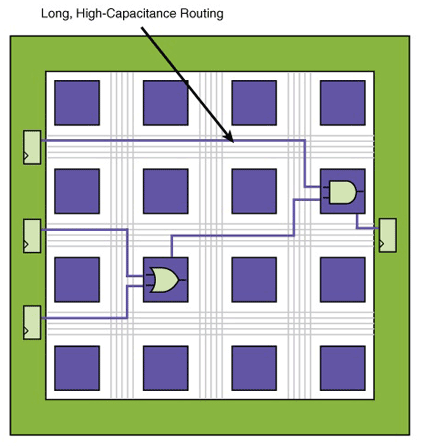
\includegraphics[width=0.40\textwidth]{img/fpga/exemploInicial.png}
				\caption{Exemplo de roteamento interno.}
				\label{fig:exemploInicial}
			\end{figure}
			\columnbreak
			\begin{itemize}
				\setlength\itemsep{1em}
				\item O FPGA \textbf{não possui funções lógicas} como AND, OR...
				\begin{itemize}
					\item Seu arranjo de células reconfiguráveis permite a \textbf{implementação} dessas portas/tabelas.
				\end{itemize}

				\item Distribuições lógicas ruins e encaminhamentos mal feitos geram atrasos de processamento
				\begin{itemize}
					\setlength\itemsep{0.3em}
					\item Estudar qual a melhor maneira projetar cada circuito;

					\item A implementação afeta diretamente seu seu design e por fim, no desempenho.
				\end{itemize}

			\end{itemize}
		\end{multicols}
	\end{frame}

	\begin{frame}%{FPGA - Hardware - Roteamento de Blocos}
		\begin{figure}[h]
			\centering
			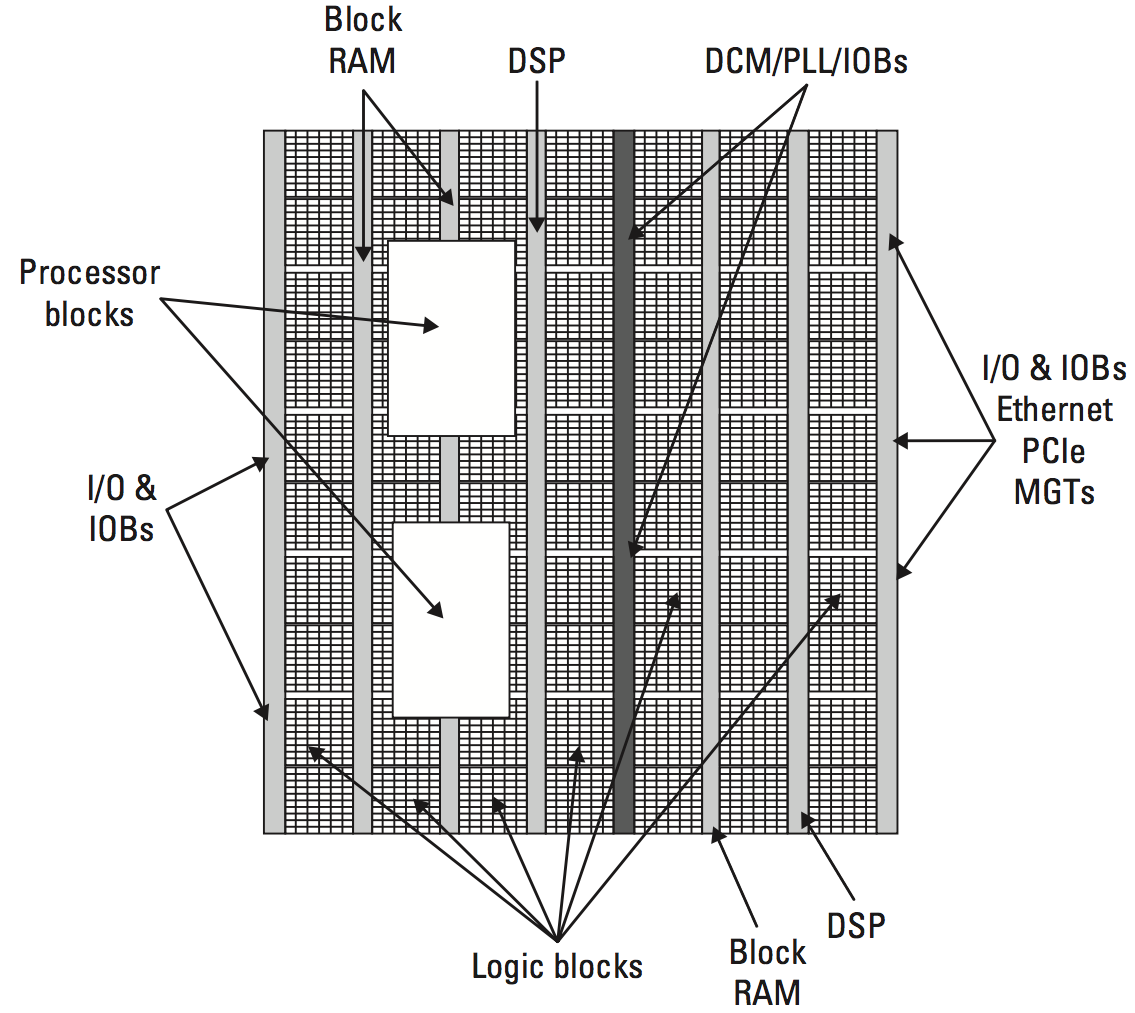
\includegraphics[height=1\textheight]{img/fpga/abstracao.png}
			\caption{Abstração de um FPGA.}
			\label{fig:abstracao}
		\end{figure}
	\end{frame}

	\begin{frame}%{FPGA - Hardware - Roteamento de Blocos}
		\begin{figure}[h]
			\centering
			\includegraphics[width=0.56\textwidth]{img/fpga/exemploFinal.png}
			\caption{Exemplo de roteamento interno complexo no FPGA.}
			\label{fig:exemploFinal}
		\end{figure}
	\end{frame}

	\begin{frame}{FPGA - Hardware - Placa}
        \vspace{-1em}
		\begin{figure}[p]
			\centering
			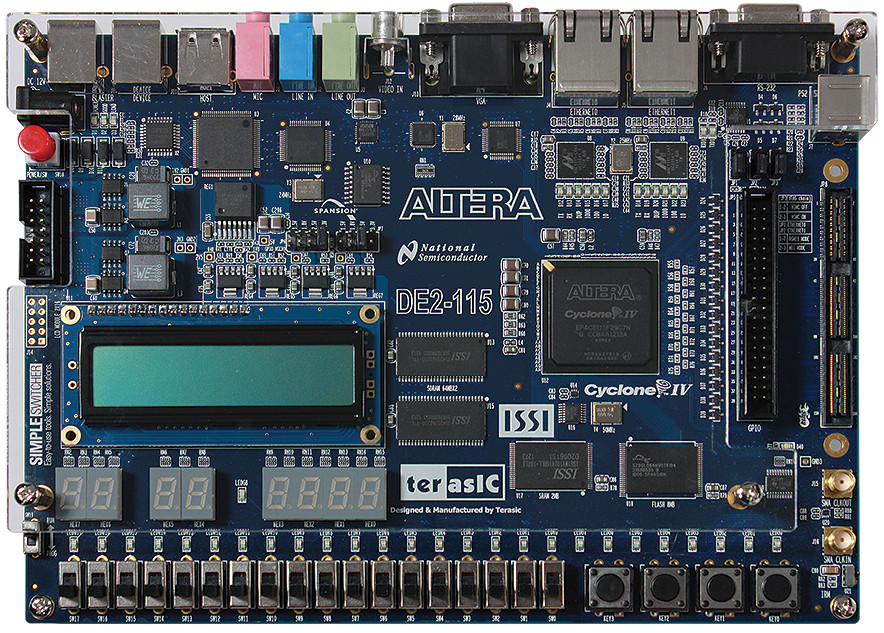
\includegraphics[width=0.64\textwidth]{img/fpga/terasic_placa.jpg}
			\caption{FPGA de Desenvolvimento Altera DE2-115.}
			\label{fig:terasic_placa}
		\end{figure}
	\end{frame}

	\begin{frame}%{FPGA - Hardware - Placa}
		\begin{figure}[p]
			\centering
			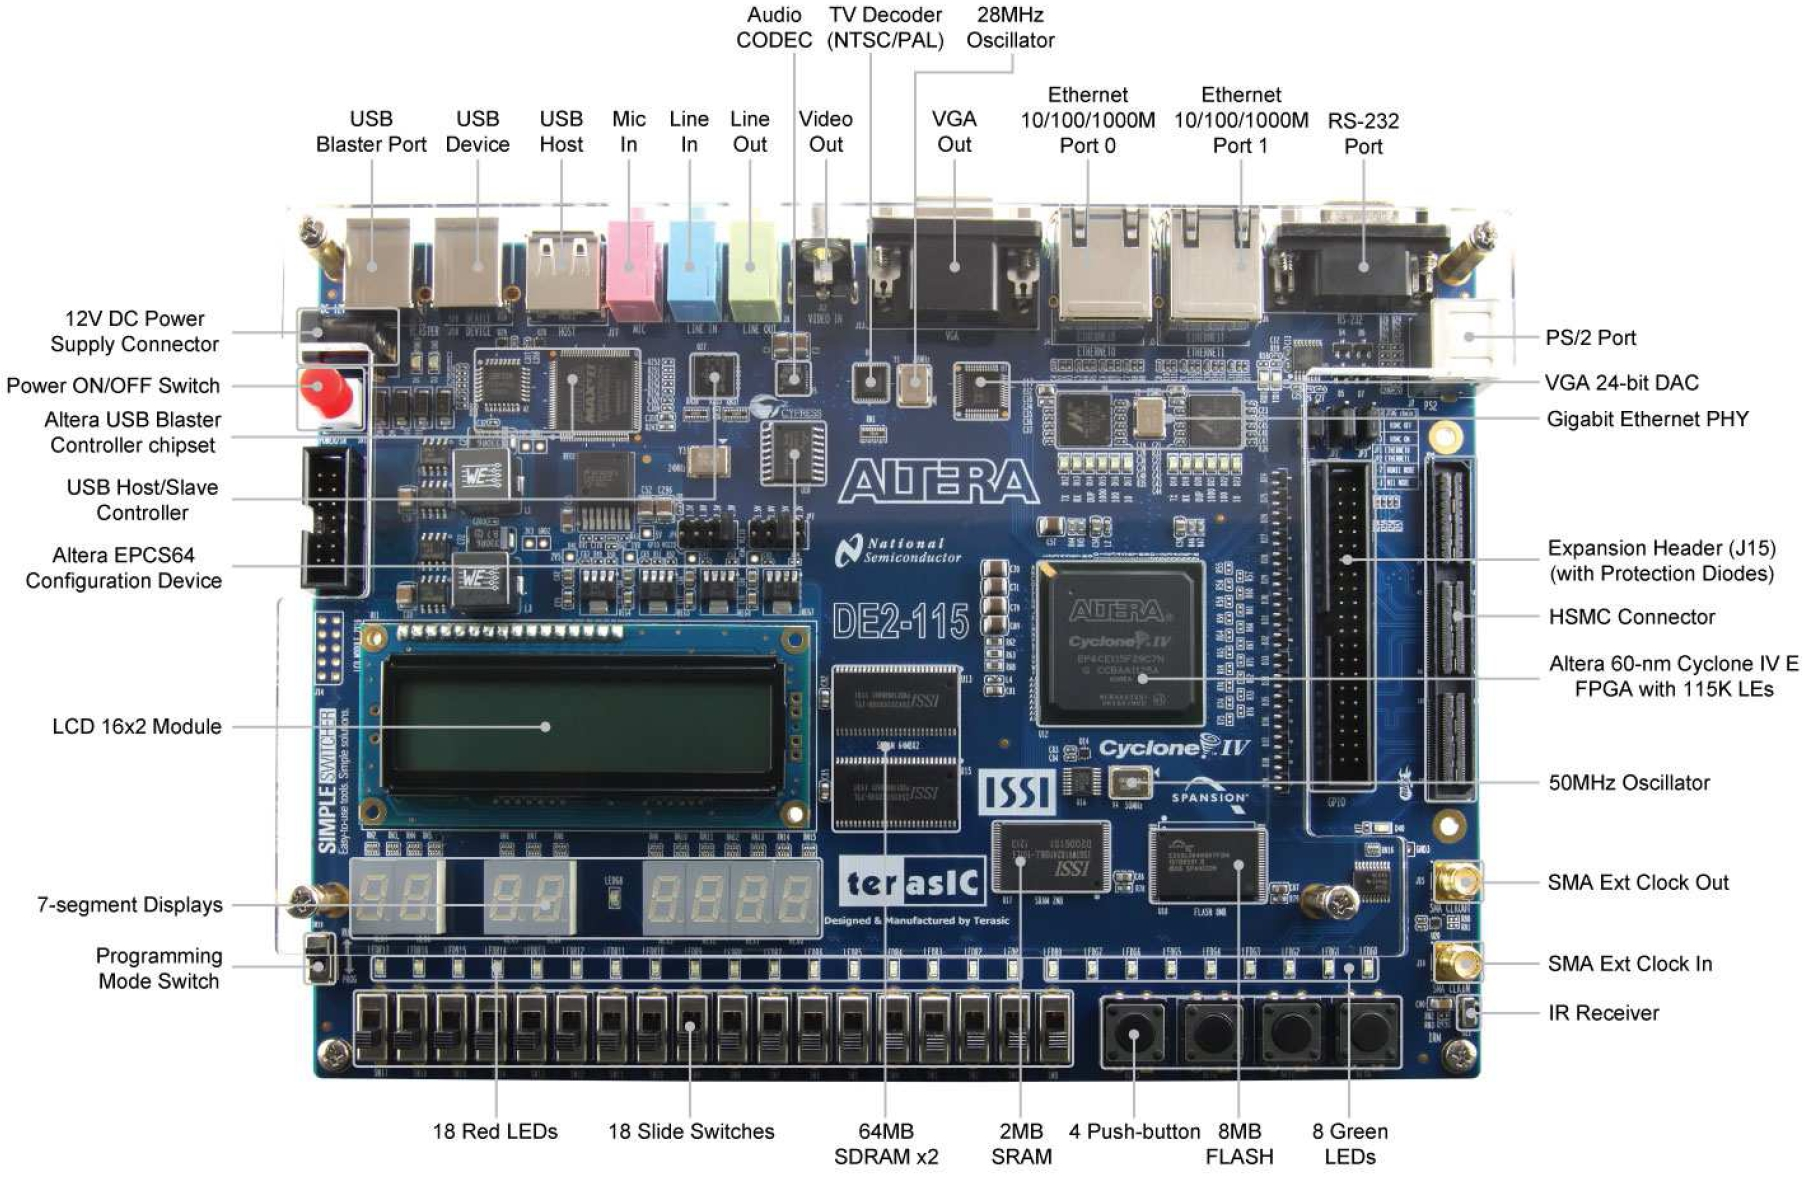
\includegraphics[width=0.9\textwidth]{img/fpga/terasic_placa_detalhado.jpg}
			\caption{FPGA de Desenvolvimento Altera DE2-115.}
			\label{fig:terasic_placa2}
		\end{figure}
	\end{frame}



\subsection{Software}
	\begin{frame}{FPGA - Software - IDE de Desenvolvimento}
        \vspace{-1em}
		\begin{figure}[p]
			\centering
			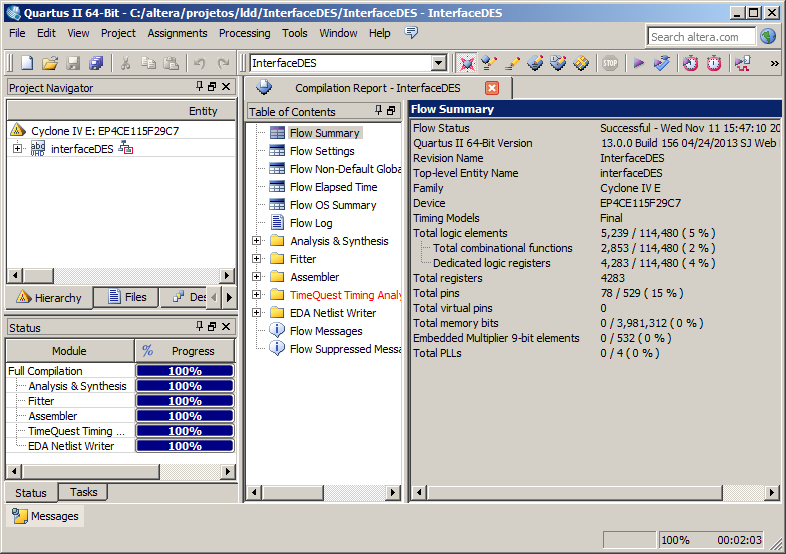
\includegraphics[width=0.8\textwidth]{img/fpga/altera.png}
			\caption{Altera Quartus II.}
			\label{fig:alteraquartus}
		\end{figure}
	\end{frame}

	\begin{frame}{FPGA - Software - IDE de Desenvolvimento}
        \vspace{-1em}
		\begin{figure}[p]
			\centering
			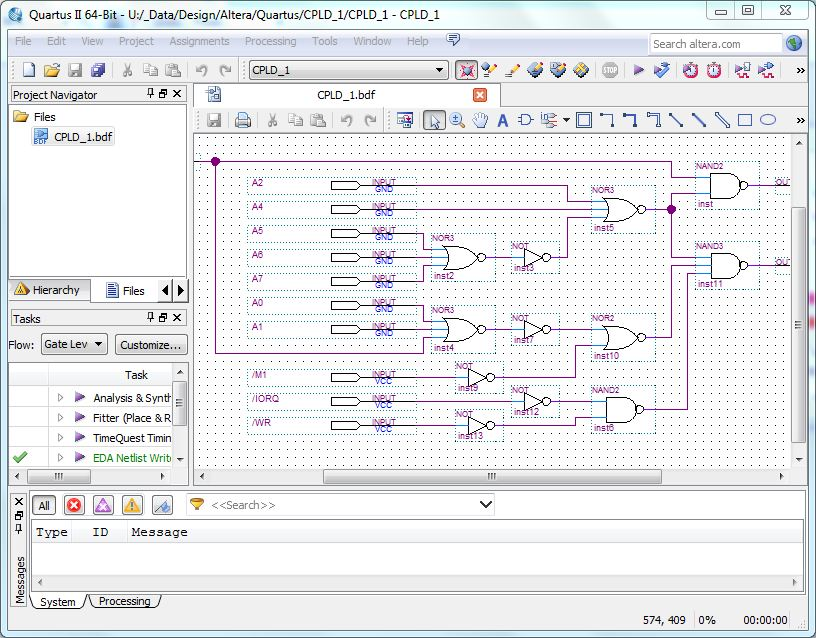
\includegraphics[width=0.63\textwidth]{img/fpga/software_quartus_portas.jpg}
			\caption{Projeto com assistência computacional usando portas lógicas.}
			\label{fig:alteraquartus_portas1}
		\end{figure}
	\end{frame}

	\begin{frame}{FPGA - Software - IDE de Desenvolvimento}
        \vspace{-1em}
		\begin{figure}[p]
			\centering
			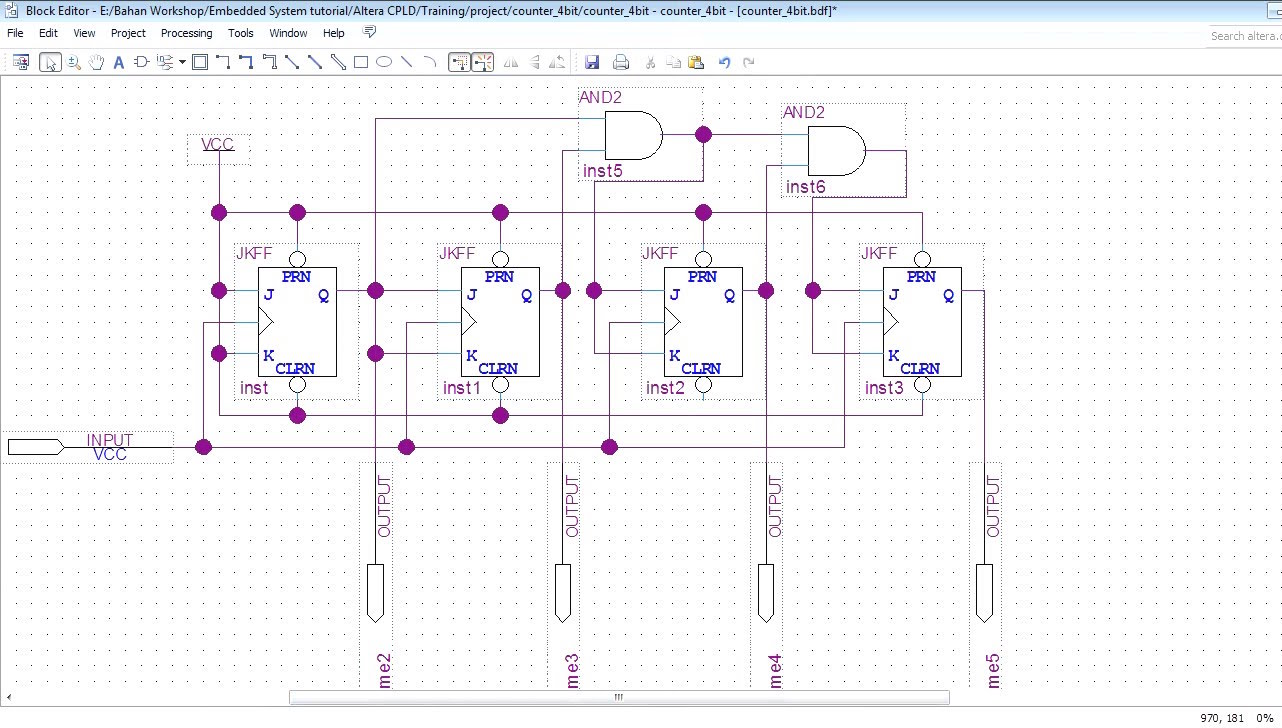
\includegraphics[width=0.85\textwidth]{img/fpga/software_quartus_portas2.jpg}
			\caption{Projeto Contador 4-bit usando portas lógicas.}
			\label{fig:alteraquartus_portas2}
		\end{figure}
	\end{frame}

	\begin{frame}{FPGA - Software - IDE de Desenvolvimento}
        \vspace{-1em}
		\begin{figure}[p]
			\centering
			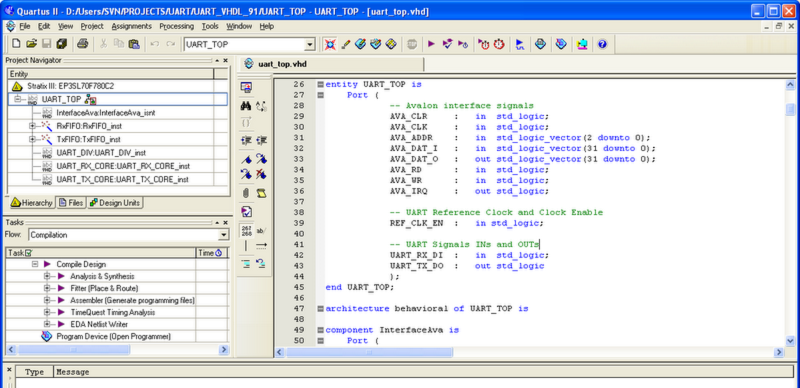
\includegraphics[width=1\textwidth]{img/fpga/software_quartus_vhdl.png}
			\caption{Projeto de uma interface UART usando VHDL.}
			\label{fig:alteraquartus_portas}
		\end{figure}
	\end{frame}

	\begin{frame}{FPGA - Software - IDE de Desenvolvimento}
		\begin{figure}[p]
			\centering
			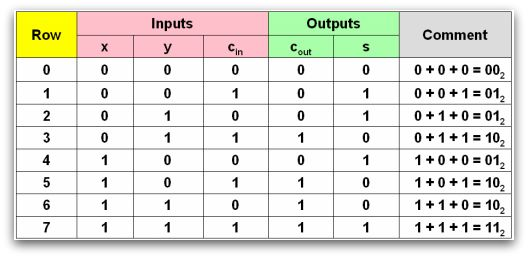
\includegraphics[width=1\textwidth]{img/fpga/adder-table.jpg}
			\caption{Somador Completo.}
			\label{fig:somador_completo}
		\end{figure}
	\end{frame}

	\begin{frame}{FPGA - Software - IDE de Desenvolvimento}
		\begin{figure}[p]
			\centering
			
\includegraphics[width=0.77\textwidth]{img/fpga/adder.png}
			\caption{Representação do Somador Completo em Portas Lógicas.}
			\label{fig:somador_completo_pl}
		\end{figure}
	\end{frame}

	\begin{frame}%{FPGA - Software - IDE de Desenvolvimento}
		\begin{figure}[p]
			\centering
			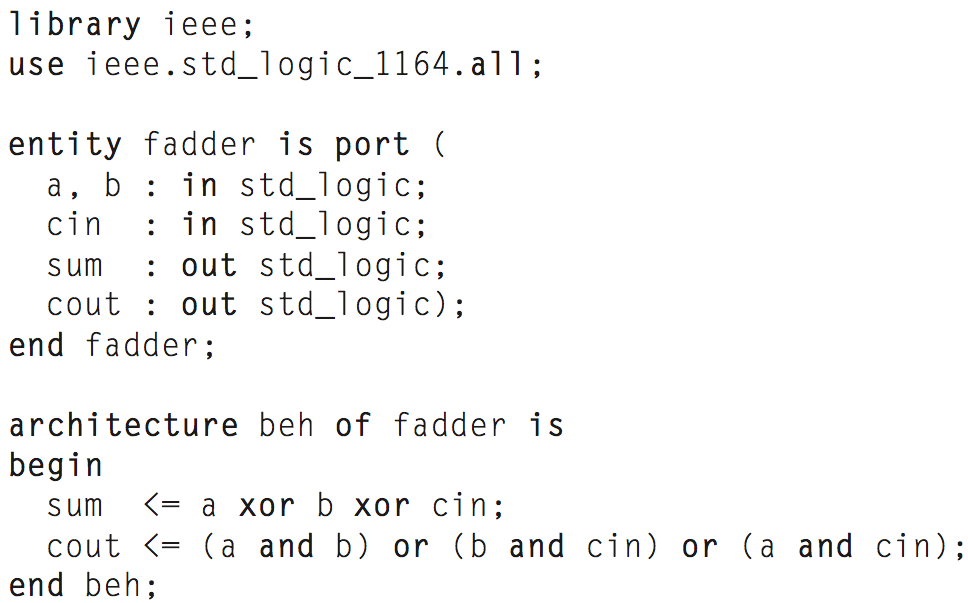
\includegraphics[width=0.8\textwidth]{img/fpga/code_vhdl.png}
			\caption{Código do Somador Completo em VHDL.}
			\label{fig:codigo_vhdl}
		\end{figure}
	\end{frame}


	\begin{frame}{FPGA - Software - IDE de Desenvolvimento}
		\begin{figure}[p]
			\centering
			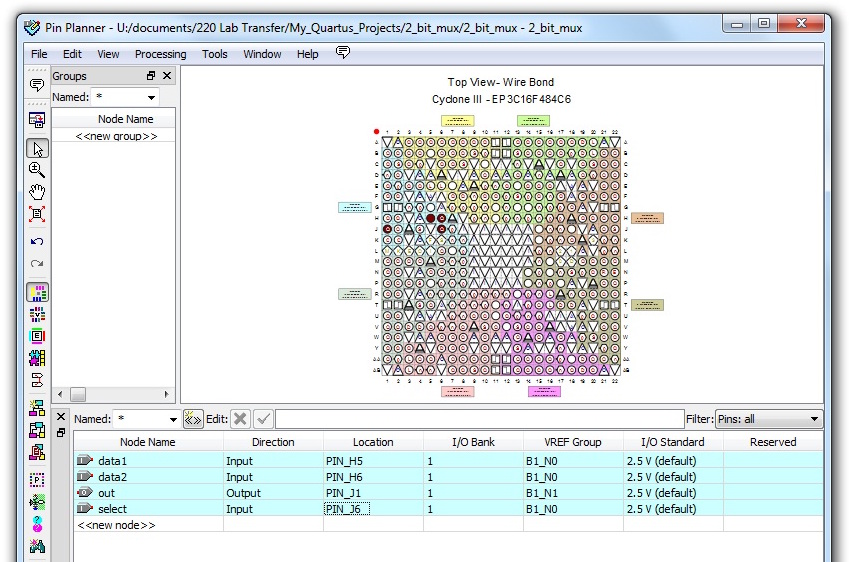
\includegraphics[width=0.74\textwidth]{img/fpga/software_quartus_pin.jpg}
			\caption{Pin Planner.}
			\label{fig:alteraquartus_pinagem}
		\end{figure}
	\end{frame}

	\begin{frame}%{FPGA - Software - IDE de Desenvolvimento}
		\begin{figure}[p]
			\centering
			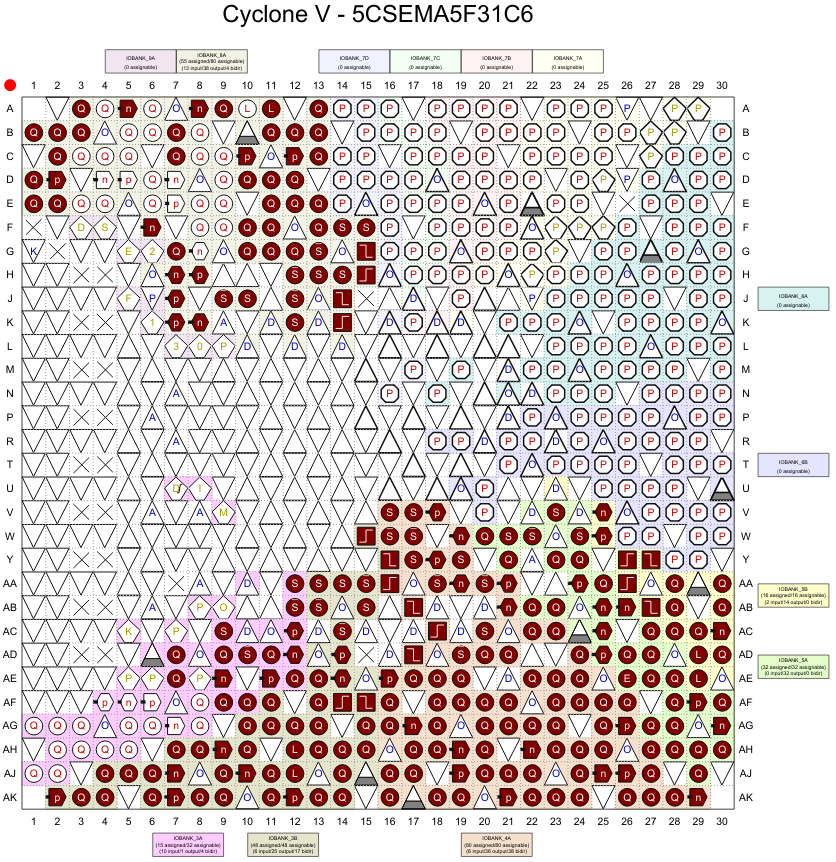
\includegraphics[width=0.56\textwidth]{img/fpga/pinplanner.png}
			\caption{Pin Planner aproximado.}
			\label{fig:pinplanner}
		\end{figure}
	\end{frame}

	\begin{frame}{FPGA - Software - IDE de Desenvolvimento}
		\begin{figure}[p]
			\centering
			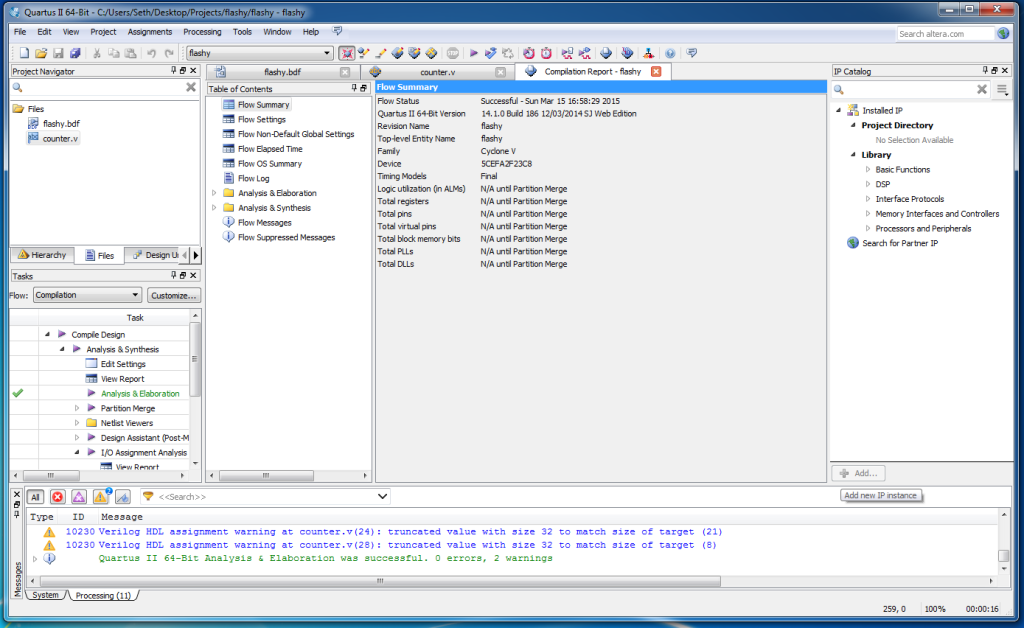
\includegraphics[width=0.8\textwidth]{img/fpga/software_quartus_compilation0.png}
			\caption{Início de síntese de um projeto.}
			\label{fig:alteraquartus_comp0}
		\end{figure}
	\end{frame}

	\begin{frame}{FPGA - Software - IDE de Desenvolvimento}
		\begin{figure}[p]
			\centering
			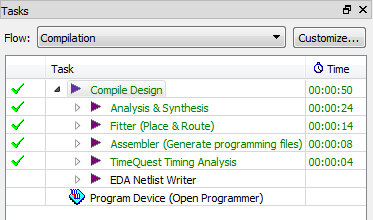
\includegraphics[width=0.8\textwidth]{img/fpga/software_quartus_compilation1.png}
			\caption{Término de síntese de um projeto.}
			\label{fig:alteraquartus_comp1}
		\end{figure}
	\end{frame}

	\begin{frame}{FPGA - Software - IDE de Desenvolvimento}
		\begin{figure}[p]
			\centering
			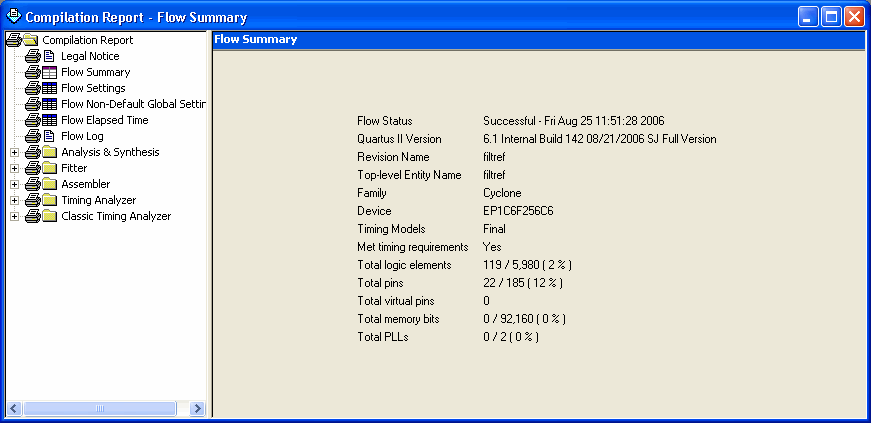
\includegraphics[width=1\textwidth]{img/fpga/software_quartus_compilation2.png}
			\caption{Relatório de compilação final.}
			\label{fig:alteraquartus_comp2}
		\end{figure}
	\end{frame}

	\begin{frame}{FPGA - Software - IDE de Desenvolvimento}
		\begin{figure}[p]
			\centering
			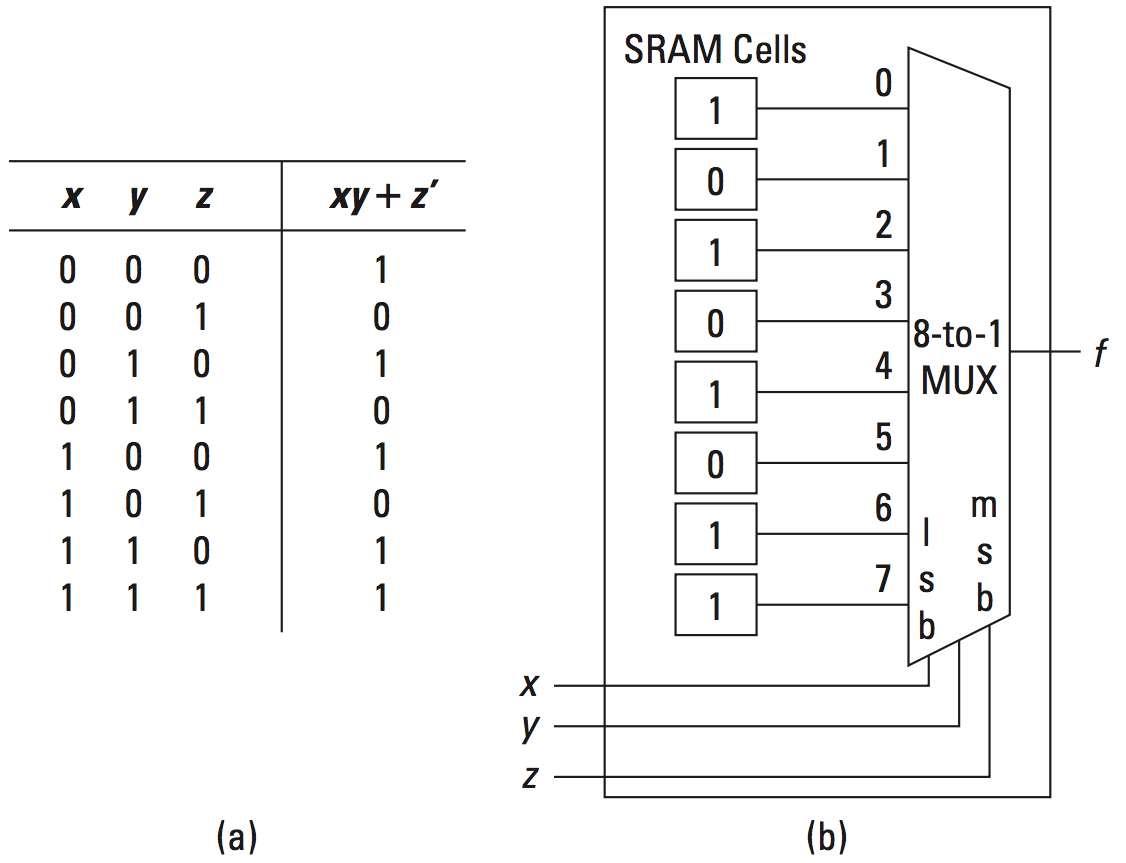
\includegraphics[width=0.58\textwidth]{img/fpga/funcao-geradora.png}
			\caption{Gerador de Função. a) tabela verdade e b) Look-Up Table (LUT) com Flip-flops para armazenamento.}
			\label{fig:funcao-geradora}
		\end{figure}
	\end{frame}




	\begin{frame}{FPGA - Software - IDE de Simulação}
		\begin{figure}[p]
			\centering
			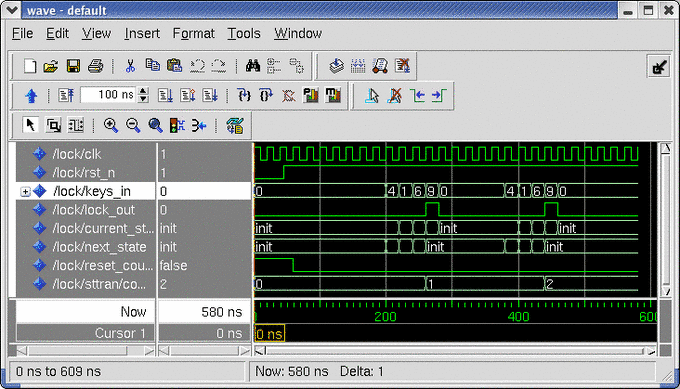
\includegraphics[width=0.85\textwidth]{img/fpga/modelsim.png}
			\caption{ModelSim.}
			\label{fig:modelsim}
		\end{figure}
	\end{frame}



\subsection{Programação}
\begin{frame}{FPGA - Programação}
	\begin{itemize}
		\setlength\itemsep{1.0em}
		\item A implementação na placa FPGA é feita por:
		\begin{itemize}
			\setlength\itemsep{0.5em}
			\item Linguagens de descrição chamadas de \textbf{Linguagens de Descrição de \textit{Hardware} (HDL)}
			\begin{itemize}
				\item São algumas linguagens: VHDL \textit{(foto)}, Verilog, ABEL, etc..
			\end{itemize}

			\item Ou por meio do desenvolvimento de \textbf{diagramas esquemáticos com ferramentas gráficas assistidas pelo computador} \textit{(foto)}.

			\item Hoje, também é possível escrever por meio de \textbf{linguagens de alto nível} para como Handel-C, C-like ou mesmo o SystemC.
		\end{itemize}

		\item Alguns conceitos de fundamentais sobre linguagens de descrição de \textit{hardware}:
		\begin{itemize}
			\setlength\itemsep{0.5em}
			\item Estas linguagens permitem por exemplo \textit{loops} infinitos ou portas lógicas com inúmeras entradas;

			\item Essas são possível serem descritas em \textit{software} mas impossível de implementar em \textit{hardware}.
		\end{itemize}
	\end{itemize}
\end{frame}

	\begin{frame}{FPGA - Programação}
		\begin{figure}[p]
			\centering
			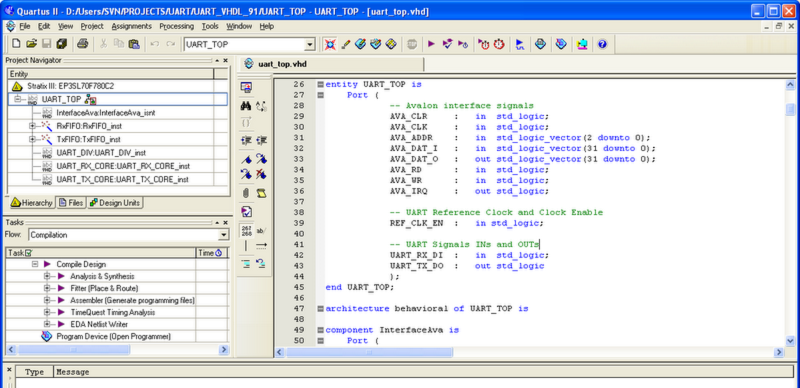
\includegraphics[width=1\textwidth]{img/fpga/software_quartus_vhdl.png}
			\caption{Projeto de uma interface UART usando VHDL.}
			\label{fig:alteraquartus_vhdl-2}
		\end{figure}
	\end{frame}

	\begin{frame}{FPGA - Programação}
		\begin{itemize}
			\setlength\itemsep{1.0em}
			\item A implementação na placa FPGA é feita por:
			\begin{itemize}
				\setlength\itemsep{0.5em}
				\item Linguagens de descrição chamadas de \textbf{Linguagens de Descrição de \textit{Hardware} (HDL)}
				\begin{itemize}
					\item São algumas linguagens: VHDL, Verilog, ABEL, etc..
				\end{itemize}

				\item Ou por meio do desenvolvimento de \textbf{diagramas esquemáticos com ferramentas gráficas assistidas pelo computador}.

				\item Hoje, também é possível escrever por meio de \textbf{linguagens de alto nível} para como Handel-C ou mesmo o SystemC.
			\end{itemize}

			\item Alguns conceitos de fundamentais sobre linguagens de descrição de \textit{hardware}:
			\begin{itemize}
				\setlength\itemsep{0.5em}
				\item Estas linguagens permitem por exemplo \textit{loops} infinitos ou portas lógicas com inúmeras entradas;

				\item Essas são possível serem descritas em \textit{software} mas impossível de implementar em \textit{hardware}.
			\end{itemize}
		\end{itemize}
	\end{frame}

	\begin{frame}{FPGA - Programação}
		\begin{figure}[p]
			\centering
			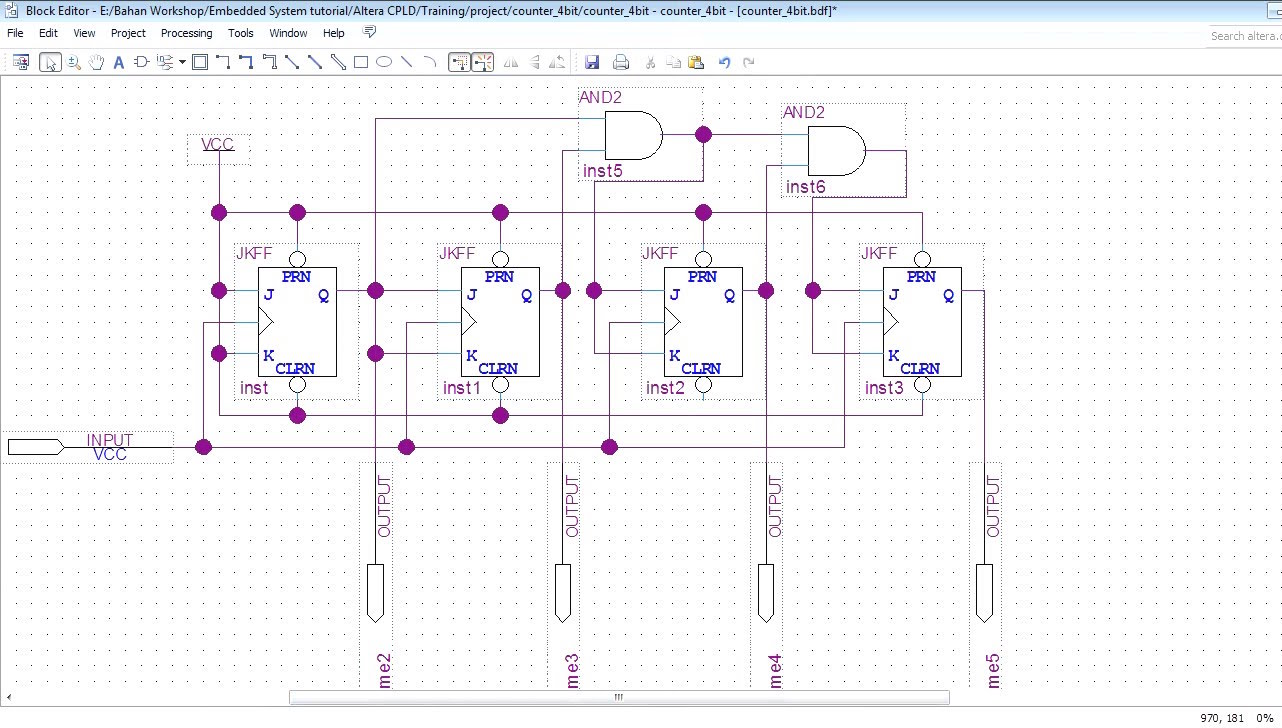
\includegraphics[width=0.85\textwidth]{img/fpga/software_quartus_portas2.jpg}
			\caption{Projeto Contador 4-bit usando portas lógicas.}
			\label{fig:alteraquartus_portas2-2}
		\end{figure}
	\end{frame}

	\begin{frame}{FPGA - Programação}
		\begin{itemize}
			\setlength\itemsep{1.0em}
			\item A implementação na placa FPGA é feita por:
			\begin{itemize}
				\setlength\itemsep{0.5em}
				\item Linguagens de descrição chamadas de \textbf{Linguagens de Descrição de \textit{Hardware} (HDL)}
				\begin{itemize}
					\item São algumas linguagens: VHDL, Verilog, ABEL, etc..
				\end{itemize}

				\item Ou por meio do desenvolvimento de \textbf{diagramas esquemáticos com ferramentas gráficas assistidas pelo computador}.

				\item Hoje, também é possível escrever por meio de \textbf{linguagens de alto nível} para como Handel-C ou mesmo o SystemC.
			\end{itemize}

			\item Alguns conceitos de fundamentais sobre linguagens de descrição de \textit{hardware}
			\begin{itemize}
				\setlength\itemsep{0.5em}
				\item Estas linguagens permitem por exemplo \textit{loops} infinitos ou portas lógicas com inúmeras entradas;

				\item Essas são possível serem descritas em \textit{software} mas impossível de implementar em \textit{hardware}.
			\end{itemize}
		\end{itemize}
	\end{frame}




	\begin{frame}{FPGA - Programação - VHDL}
		\begin{itemize}
			\setlength\itemsep{1.3em}
			\item Linguagem para descrever o \textbf{comportamento} e \textbf{estrutura} de um sistema digital.

			\item A abreviatura VHDL significa \textit{\underline{VHSIC Hardware Description Language}}
			\begin{itemize}
				\item Sendo que VHSIC significa \textit{\underline{Very High Speed Integrated Circuit}}.
			\end{itemize}

			\item Ou seja, seu nome em português é \textbf{Linguagem de Descrição de \textit{Hardware} de Circuitos Integrados com Altíssima Velocidade}.

			\item Ela tem propriedades suficientes para ser \textbf{independente tecnologicamente}
			\begin{itemize}
				\item Ou seja, a mesma linguagem VHDL utilizada para descrever as tecnologias de hoje, poderá descrever as futuras tecnologias \cite{Roth1998}.
			\end{itemize}
		\end{itemize}
	\end{frame}


	\begin{frame}[fragile]{FPGA - Programação - VHDL}
		\begin{minted}[mathescape,linenos, numbersep=5pt, gobble=2, tabsize=3, frame=lines, framesep=2mm]{vhdl}
		C <= A and B;
		E <= C or D;
		\end{minted}
		\pause
		\begin{figure}[h]
			\centering
			\caption{Altera Cyclone IV acoplado à placa da Terasic Altera DE2-115}
			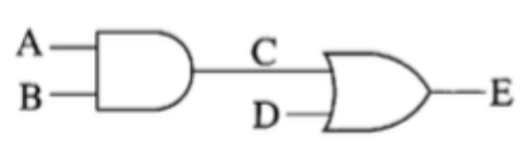
\includegraphics[height=0.2\textheight]{img/fpga/vhdl.png}
			\label{fig:vhdl}
		\end{figure}
\end{frame}

	\begin{frame}{FPGA - Bibliografia}
		\begin{multicols}{2}
			\begin{figure}[p]
				\centering
				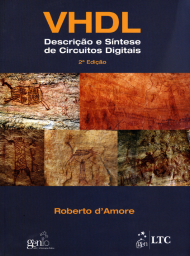
\includegraphics[width=0.3\textwidth]{img/fpga/l4.png}
				\caption{VHDL: Descrição e síntese de circuitos digitais \cite{DAmore2005}.}
				\label{fig:l4}
			\end{figure}
			\columnbreak
			\begin{figure}[p]
				\centering
				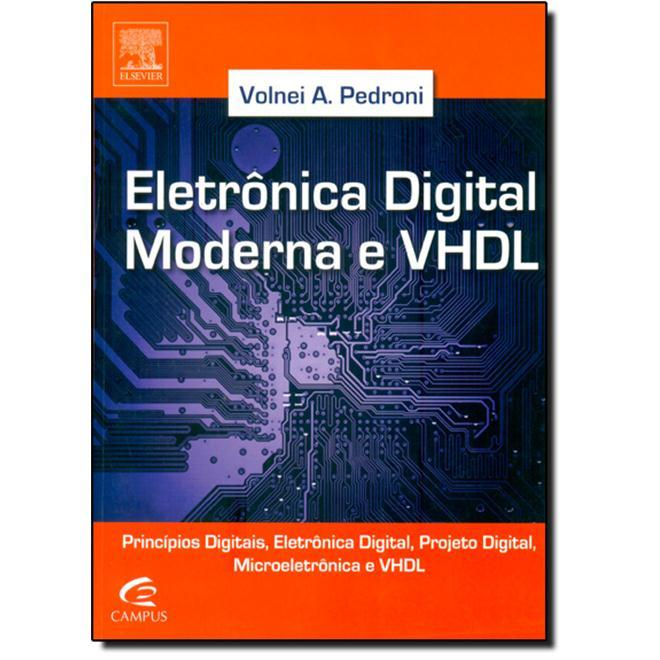
\includegraphics[width=0.43\textwidth]{img/fpga/l5.jpg}
				\caption{Eletrônica Digital Moderna e VHDL.  \cite{PEDRONI2010}.}
				\label{fig:l5}
			\end{figure}
		\end{multicols}
	\end{frame}


	\begin{frame}{FPGA - Bibliografia}
		\begin{figure}[p]
			\centering
			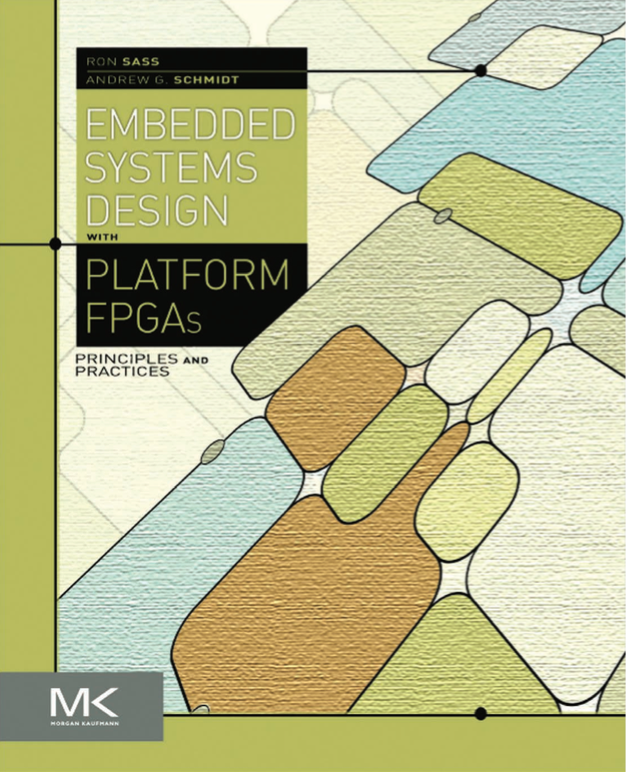
\includegraphics[width=0.35\textwidth]{img/fpga/l6.png}
			\caption{\textit{Embedded Systems Design with Platform FPGAs,
				Principles and Practices} \cite{Sass2010} .}
			\label{fig:l6}
		\end{figure}
	\end{frame}


	\begin{frame}{FPGA - Vantagens e Desvantagens}
		\begin{itemize}
			\item Vantagens:
			\begin{itemize}
				\setlength\itemsep{0.2em}
				\item Não é necessário uma ASIC pra realizar testes:
				\begin{itemize}
					\item Com o uso do FPGA, é possível fazer os testes necessários prevendo erros;
				\end{itemize}

				\item É possível adicionar mais recursos em sua placa para que o projeto tente simular o mais próximo possível do produto final
				\begin{itemize}
					\item Câmeras, telas \textit{touch} ...
				\end{itemize}

				\item Amplamente usado para didática para a construção de circuitos integrados;

				\item Aplicação em diversas áreas inclusive áreas de grande importância como projetos no qual necessita de sistema críticos
				\begin{itemize}
					\item A Nasa...
					\item A Intel... \textit{(foto)}
				\end{itemize}
			\end{itemize}

				\bigskip

			\item Desvantagens:
			\begin{itemize}
				\setlength\itemsep{0.2em}
				\item Seu custo é bastante elevado para a utilização em projetos pequenos;

				\item Ele não possui capacidade de usar recurso analógicos;

				\item Seu desempenho entra em desvantagem em comparação com placas ASIC.
			\end{itemize}
		\end{itemize}
	\end{frame}

	\begin{frame}
		\begin{figure}[H]
			\centering
			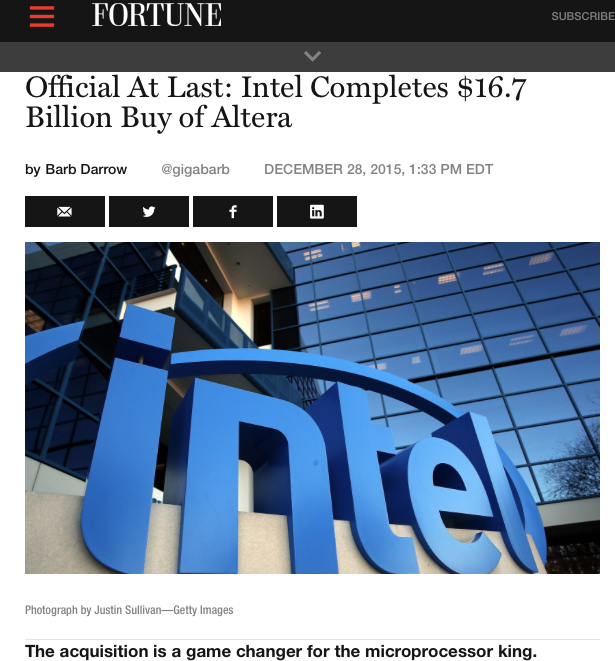
\includegraphics[width=0.48\textwidth]{img/fpga/intel_altera_2.png}
			\protect\caption{Noticiário. Fonte: \url{http://fortune.com/2015/12/28/intel-completes-altera-acquisition/}}
			\label{fig:intel_altera_noticia}
		\end{figure}
	\end{frame}

	\begin{frame}{FPGA - Vantagens e Desvantagens}
		\begin{itemize}
			\item Vantagens:
			\begin{itemize}
				\setlength\itemsep{0.2em}
				\item Não é necessário uma ASIC pra realizar testes:
				\begin{itemize}
					\item Com o uso do FPGA, é possível fazer os testes necessários prevendo erros;
				\end{itemize}

				\item É possível adicionar mais recursos em sua placa para que o projeto tente simular o mais próximo possível do produto final
				\begin{itemize}
					\item Câmeras, telas \textit{touch} ...
				\end{itemize}

				\item Amplamente usado para didática para a construção de circuitos integrados;

				\item Aplicação em diversas áreas inclusive áreas de grande importância como projetos no qual necessita de sistema críticos
				\begin{itemize}
					\item A Nasa...
					\item A Intel...
				\end{itemize}
			\end{itemize}

			\bigskip

			\item Desvantagens:
			\begin{itemize}
				\setlength\itemsep{0.2em}
				\item Seu custo é bastante elevado para a utilização em projetos pequenos;

				\item Ele não possui capacidade de usar recurso analógicos;

				\item Seu desempenho entra em desvantagem em comparação com placas ASIC.
			\end{itemize}
		\end{itemize}
	\end{frame}
